\usetikzlibrary{fit}
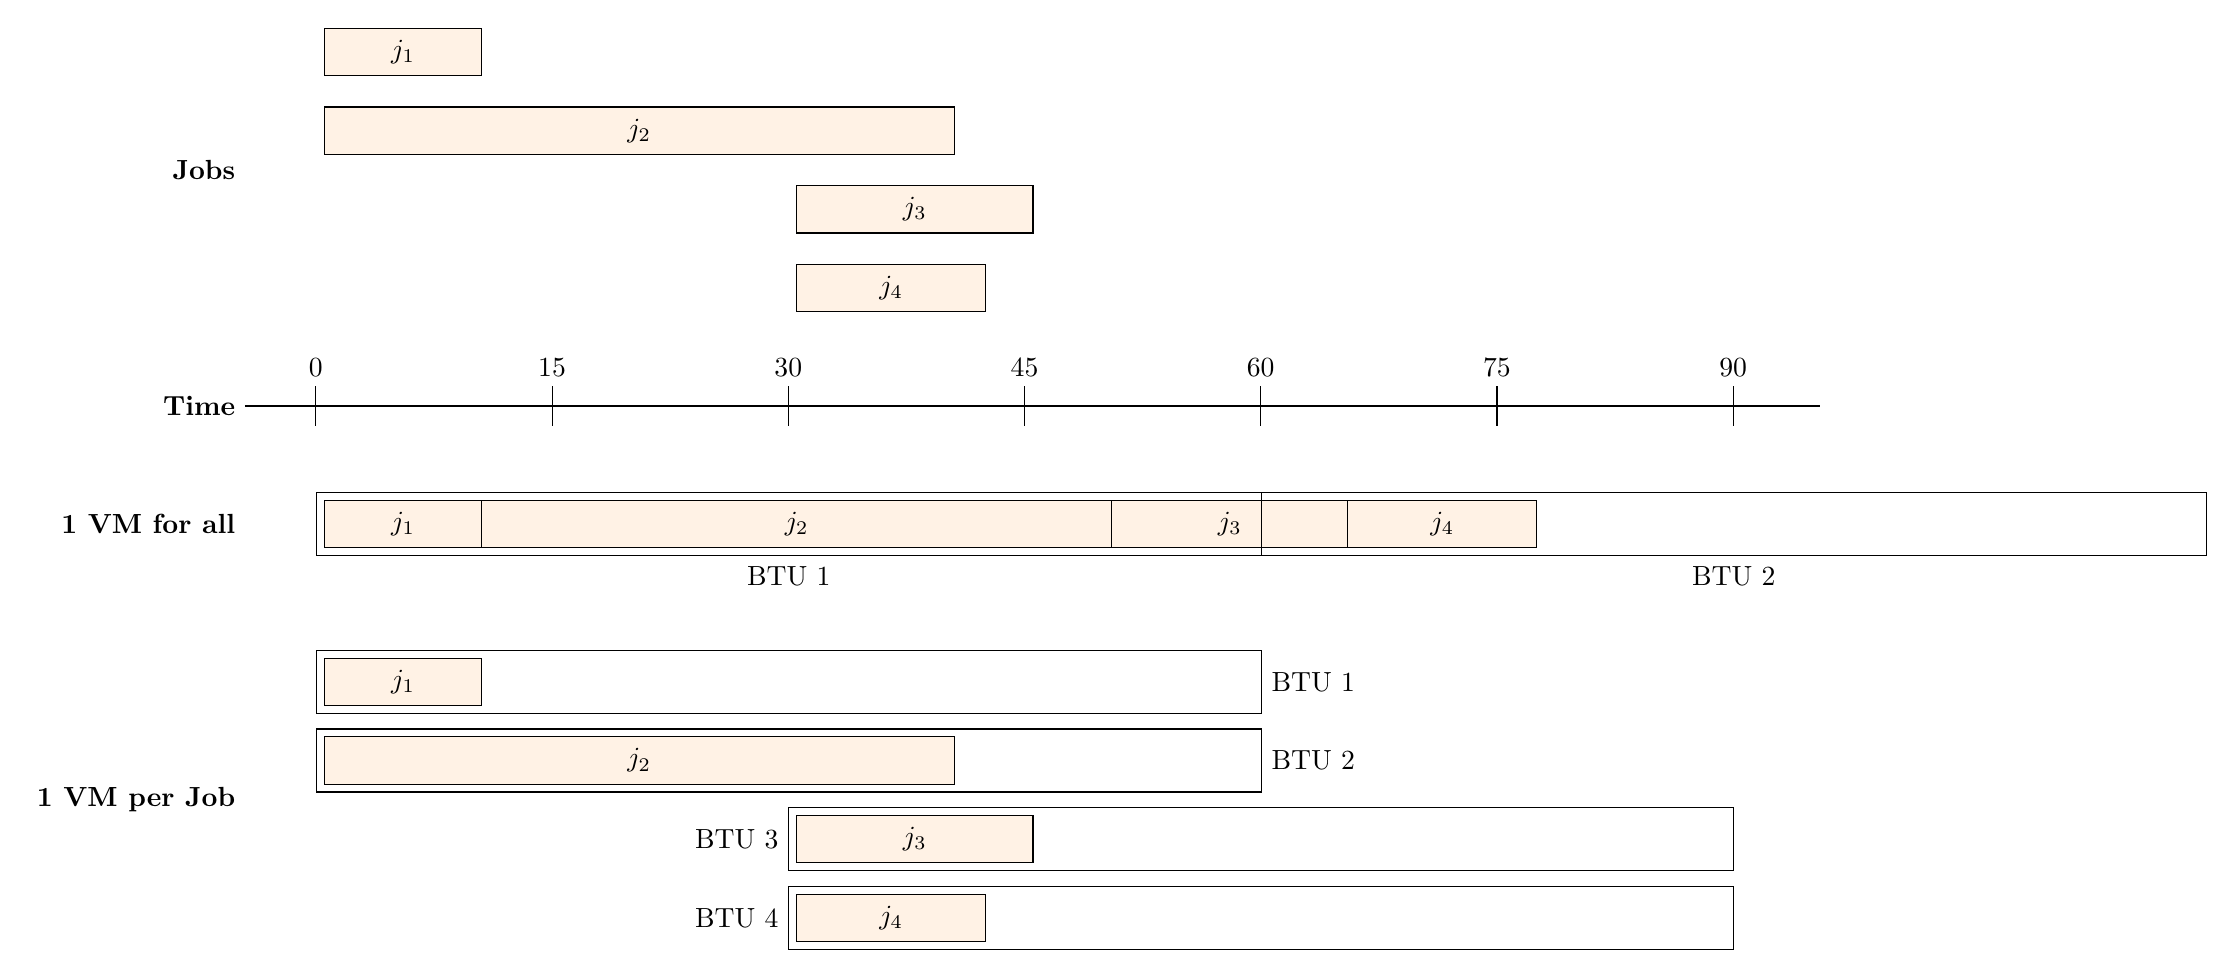
\begin{tikzpicture}[x=2mm,
job/.style={%
anchor=west,
fill=orange!10,
minimum height=6mm,
draw
},
btu/.style={%
anchor=west,
draw,
minimum height=8mm,
minimum width=120mm,
},
strat/.style={%
font=\bfseries,
anchor=east,
align=right,
},
]
%% Timeline
\node[strat]at(-5,0.5){Time};
\draw[thick] (-5,0.5)--(95,0.5);
\foreach \x in {0,15,...,90}{%
\draw (\x-0.5,0.25)--(\x-0.5,0.75) node[anchor=south]{\x};
}
%% Jobs
\node[strat]at(-5,3.5){Jobs};
\node[job,minimum width=20mm]at(0,5){$j_1$};
\node[job,minimum width=80mm]at(0,4){$j_2$};
\node[job,minimum width=30mm]at(30,3){$j_3$};
\node[job,minimum width=24mm]at(30,2){$j_4$};
%% 1vm4all
\node[strat]at(-5,-1){1 VM for all};
\node[job,minimum width=20mm]at(0,-1){$j_1$};
\node[job,minimum width=80mm]at(10,-1){$j_2$};
\node[job,minimum width=30mm]at(50,-1){$j_3$};
\node[job,minimum width=24mm]at(65,-1){$j_4$};
\node[btu,label={south:BTU 1}]at(-0.5,-1){};
\node[btu,label={south:BTU 2}]at(59.5,-1){};
%% 1VM/job
\node[strat]at(-5,-4.5){1 VM per Job};
\node[job,minimum width=20mm]at(0,-3){$j_1$};
\node[job,minimum width=80mm]at(0,-4){$j_2$};
\node[job,minimum width=30mm]at(30,-5){$j_3$};
\node[job,minimum width=24mm]at(30,-6){$j_4$};
\node[btu,label={east:BTU 1}]at(-0.5,-3){};
\node[btu,label={east:BTU 2}]at(-0.5,-4){};
\node[btu,label={west:BTU 3}]at(29.5,-5){};
\node[btu,label={west:BTU 4}]at(29.5,-6){};
\end{tikzpicture}
